% !TEX root = ../../../main.tex
% 来源：中学数学实验教材·第三册（高中数学）
% 章节：三角函数的图象和性质 / 正弦型曲线
% 原始文件：7.tex，行 1443-1469
% 类型：tikz
% ---
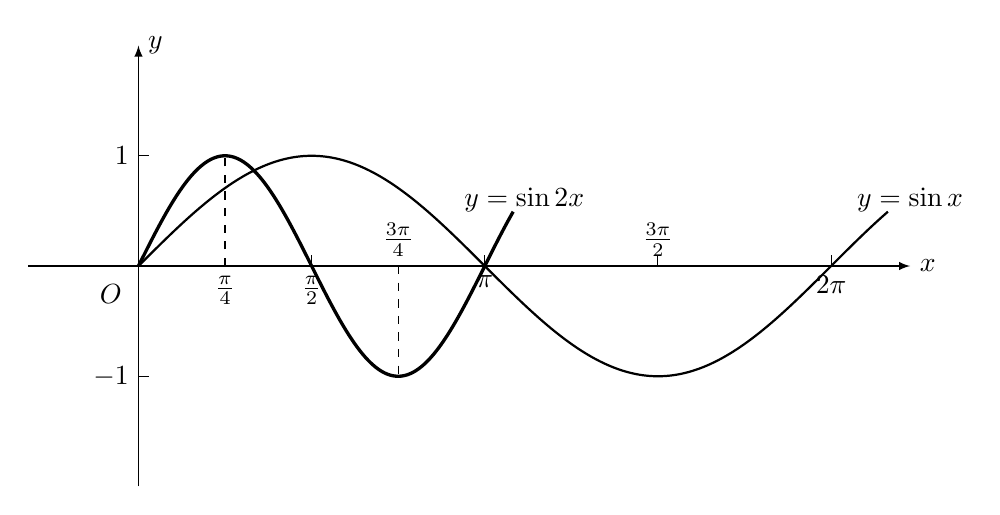
\begin{tikzpicture}[>=latex, scale=1.4]
\draw[->] (-1,0)--(7,0)node[right]{$x$};
\draw[->]  (0,-2)--(0,2)node[right]{$y$};
\draw [domain=0:6.8, samples=1000, thick] plot(\x, {sin(\x r)});
\draw [domain=0:3.4, samples=1000, very thick] plot(\x, {sin(2*\x r)});
\node at (-.25,-.25){$O$};
\foreach \x in {-1,1}
{
    \draw (0,\x)node[left]{$\x$}--(.1,\x);
}
\foreach \x in {1,2,3,4}
{
    \draw (pi*\x/2,0)--(pi*\x/2,0.1);
}
\node at (pi/2,0)[below]{$\frac{\pi}{2}$};
\node at (pi,0)[below]{$\pi$};
\node at (3*pi/2,0)[above]{$\frac{3\pi}{2}$};
\node at (2*pi,0)[below]{$2\pi$};
\node at (pi/4,0)[below]{$\frac{\pi}{4}$};
\node at (pi/4*3,0)[above]{$\frac{3\pi}{4}$};
\draw[dashed] (pi/4,0)--(pi/4,1);
\draw[dashed] (pi/4*3,0)--(pi/4*3,-1);
\node at (7,.6){$y=\sin x$};
\node at (3.5,.6){$y=\sin 2x$};


\end{tikzpicture}
